\documentclass[11pt]{article}
\usepackage{graphicx}
\usepackage{amsmath}
\usepackage{url}
\usepackage{amssymb}
\usepackage[top=1in, bottom=1in, left=0.5in, right=0.5in]{geometry}
\begin{document}
\title{CS296 Group 11 Project Report}
\author{Mayank Meghwanshi\\110050012 \\mayankmeghwanshi@gmail.com 
	\and Divyam Bansal \\ 110050086\\divyambansal93@gmail.com
	\and Jaswant Kumar \\ 110050081 \\yashwantkumar2509@gmail.com
}
\date{9th April 2013}
\maketitle

\begin{section}*{Introduction}
Purpose of this report is to display the original and final design for the Rube Goldberg Machine and state the interesting things about it. Along with this analysis of the graphs which were produced to show the relation between step time, loop time, velocity update time, position update time, collision time and the no. of iterations and re-runs is done.

\end{section}

\begin{subsection}*{Original Rube Goldberg Machine Design}
\includegraphics[width=0.7\textwidth,height=12cm,keepaspectratio]{machine.eps} 
\end{subsection}
\begin{subsection}*{Final Rube Goldberg Machine Design}
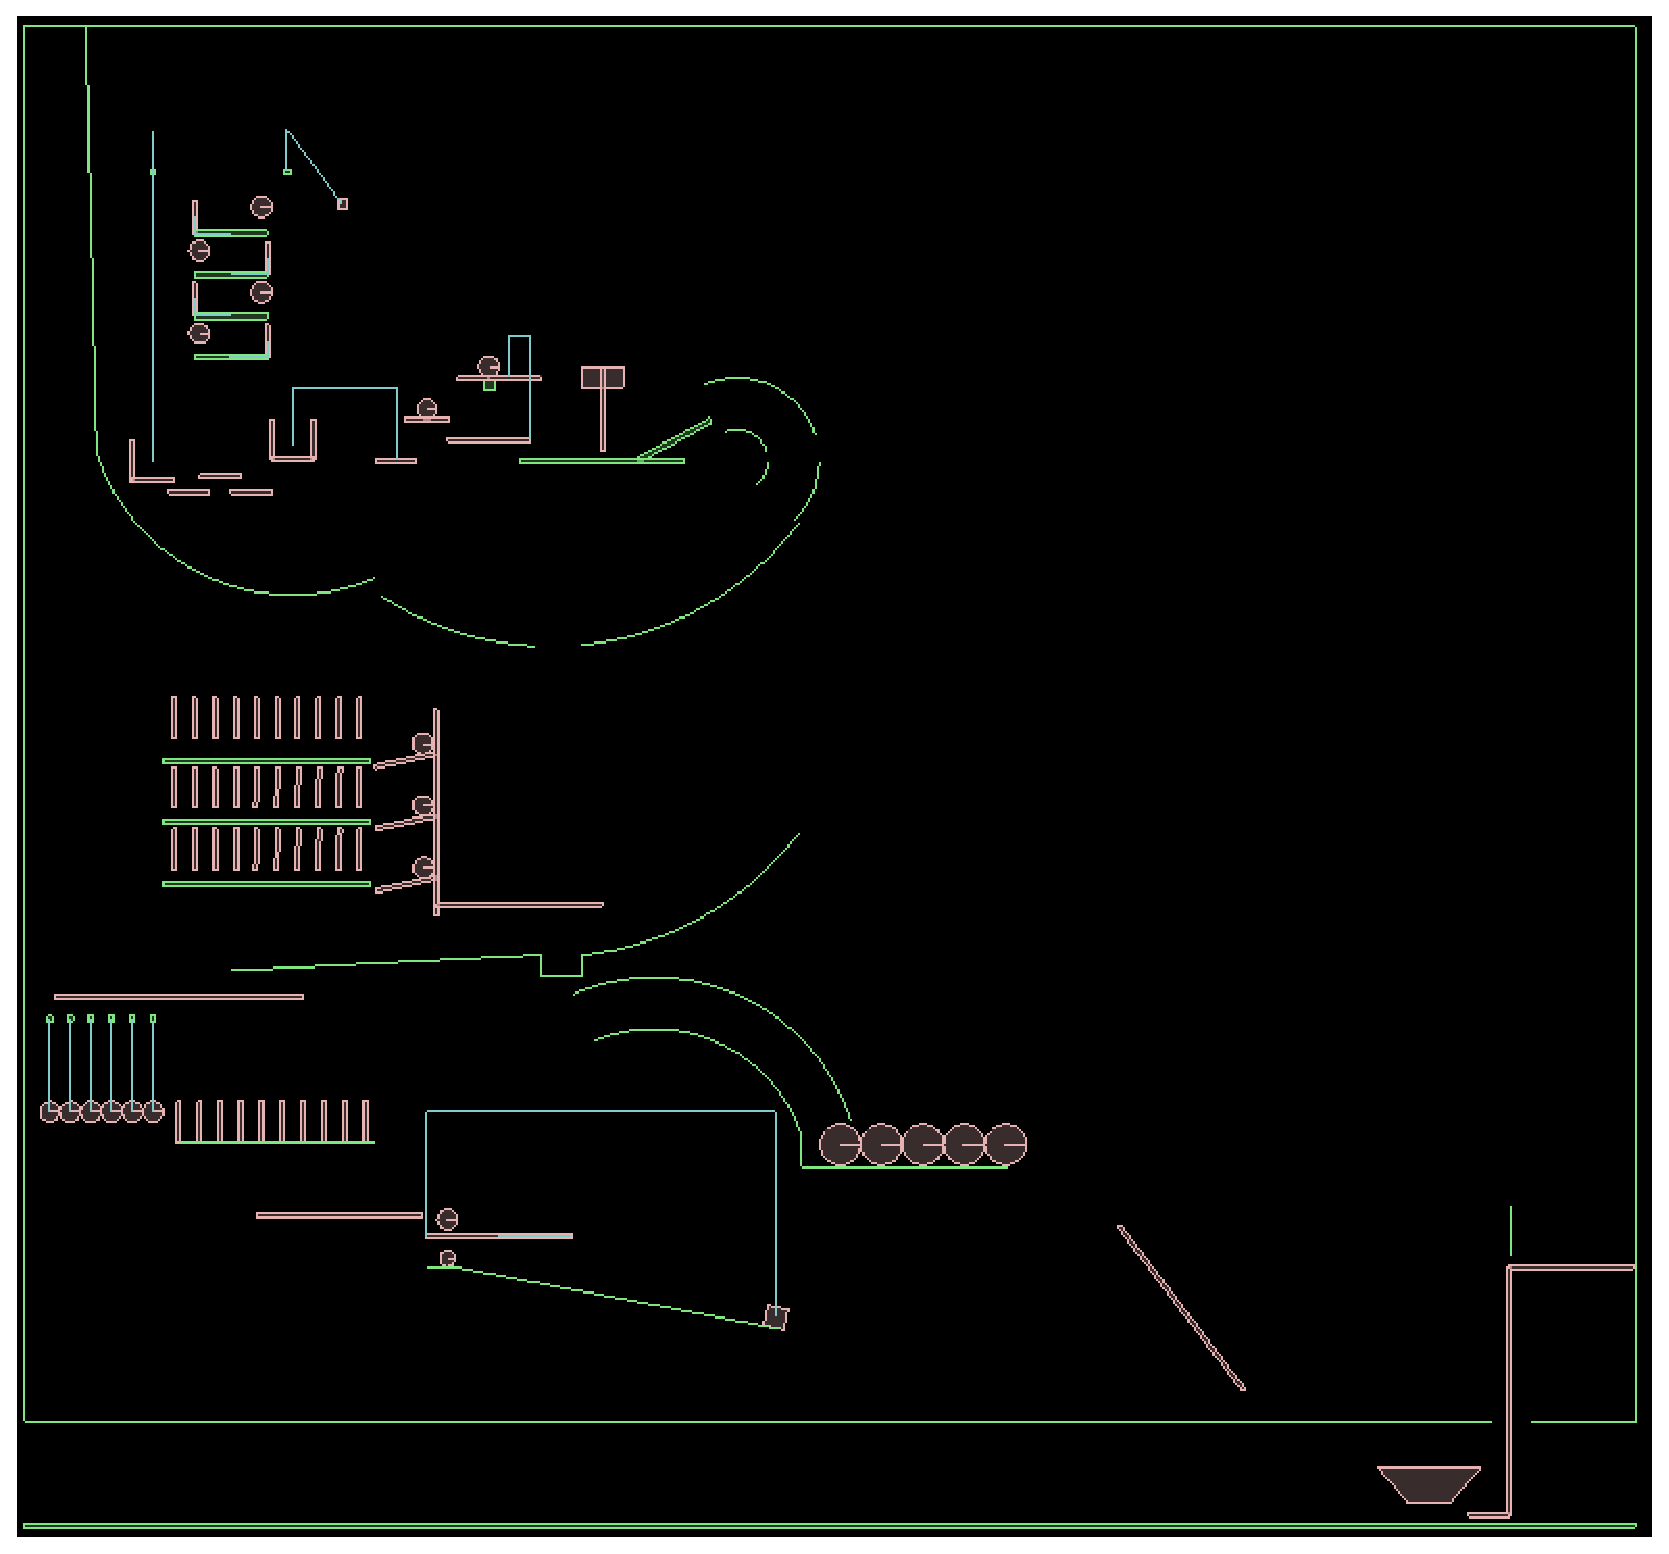
\includegraphics[width=0.7\textwidth,height=12cm,keepaspectratio]{final.eps}
\end{subsection}

\begin{subsection}*{Working of the Machine}
 Pendulum hits the ball which on rolling hits the hinged bar and ball goes on the curved surface. Hinged Bar upon rotating hits the next ball which again hits the hinged bar and itself falls into basket attached to pulley. Similarly, one balls fall in bucket on left and two balls in bucket connected to pulley. Now, puley lowers on left side and hit bar which upon rotating again hits the adjacent bar and consequently last bar hits the bucket containing ball which on moving empties itself and thus the ball fall on the surface below and rolls towards hole. When pulley lowers, bar moves up and tilts another bar resulting in the rolling of ball which falls on the next bar and itself falls on arc and than inside the hole.When ball hits the bar, pulley rotates and thus ball lowers and rolls onto the bar and hits the hammer which after rotating hits the ball from back to move the ball into the tunnel. After that this ball reaches surface and moves through the hole.
\\\\
The hole opens below and thus making the way for balls to hit bar, which moves stage of balls upwards resulting in the motion of 3 balls one by one towards dominos and consequently domino falls on rotating platform and tilts it forward to make way for the balls. Balls upon descending from bar, moves towards rotating platform and in the process three balls fall in the pit.
\\\\
Now one ball falls and hits pendulum.Pendulum moves and hits domino, resulting in domino falling on the bar below it and tilts it so that domino hits small ball, which upon moving hits the weight, and weight falls and pulls platform up and the ball on the platform flies towards the tunnel. Ball hits the Big Balls and moves them towards the motor which throws them towards fructum and tilts it. Fructum now hits the boat and moves it.
\end{subsection}


\begin{subsection}*{Differences between the Designs}
Following are the differences in our original and final design: 
\begin{itemize}
\item All the initial 4 platforms which are tilted in original design are set straight in final design, but the functionality is same. It was done otherwise balls would have rolled down under gravity.
\item A tilted platform is kept adjacent to hammer so as to provide the necessary elevation to the ball, otherwise it was difficult for the ball to rise to such height with a horizontal hit of the hammer. 
\item Only one pit is kept below the three platforms in the final design as the desired outcome was achieved with only one pit. 
\item Magnet is removed from the original design as it was very difficult to implement, it would have required the implementation of magnetic forces.
\item Certain changes are made below the series of pendulum also, because simulation in the original system was giving different outcome, so we changed it appropiately implemented a new procedure with same functionality and complexity.
\item We have replaced the spring mechanism with a rotating bar, as we were able to achieve the expected outcome from it. Also implementing a spring was a difficault task.
\item Instead of piston we have placed a lever, and the working is same as that of piston. When balls land on the top of the lever it causes its other end to lift which pushes the boat which was our final task.
\end {itemize}
\end{subsection}

\begin{subsection}*{Interesting parts in our design}
Following are the things which are intersting in our Rube Goldberg Machine:
\begin{itemize}
\item At two places tunnels are made, which are made using the parameteric equation of circle.
\item Pulley systems are kept in sequence, where one pulley triggers the other.
\item Hammer is made which hits the ball again to elevate it.
\item A rotating bar is kept which hits the big balls and forces them to fall on lever so that boat can move. 
\end{itemize}

\end{subsection}
\pagebreak
\begin{subsection}*{Timing}
\end{subsection}
\begin{subsection}*{Graph 1}
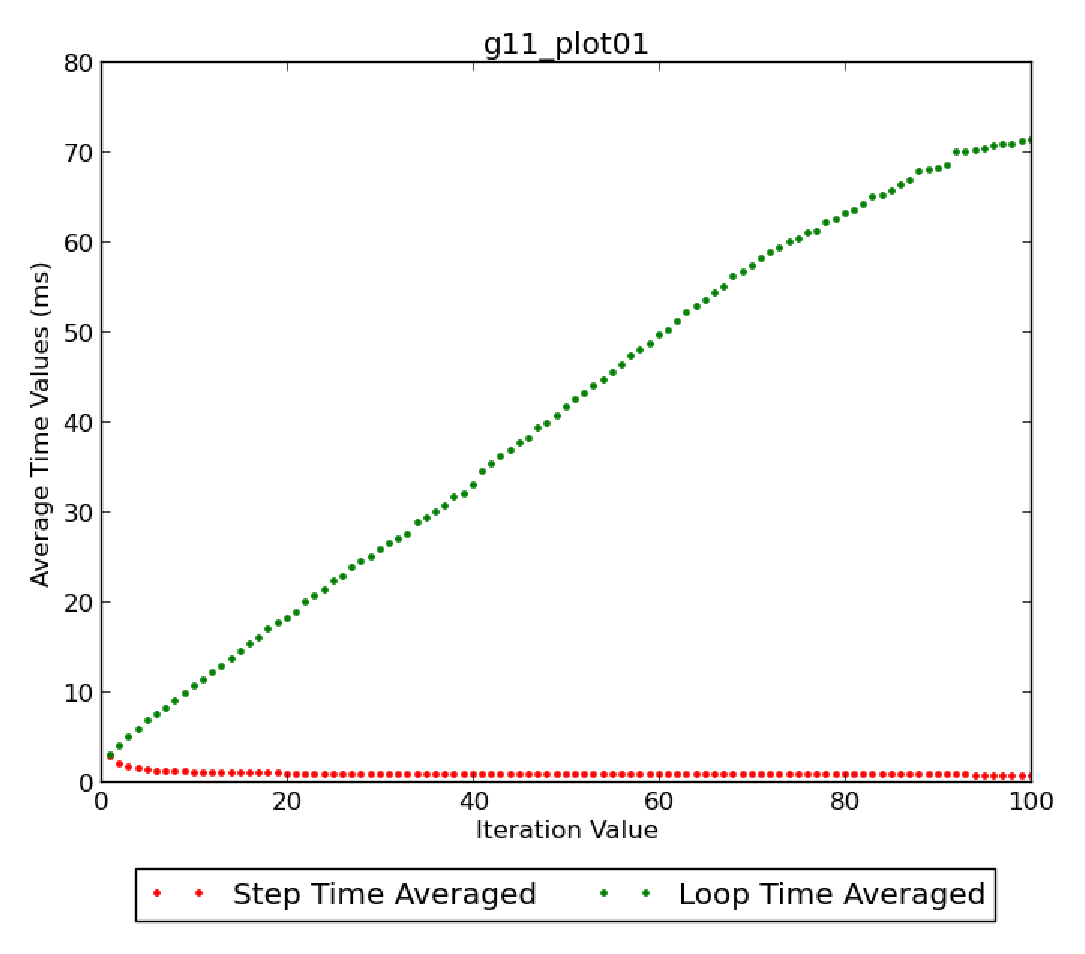
\includegraphics[width=0.5\textwidth,keepaspectratio]{1.eps} 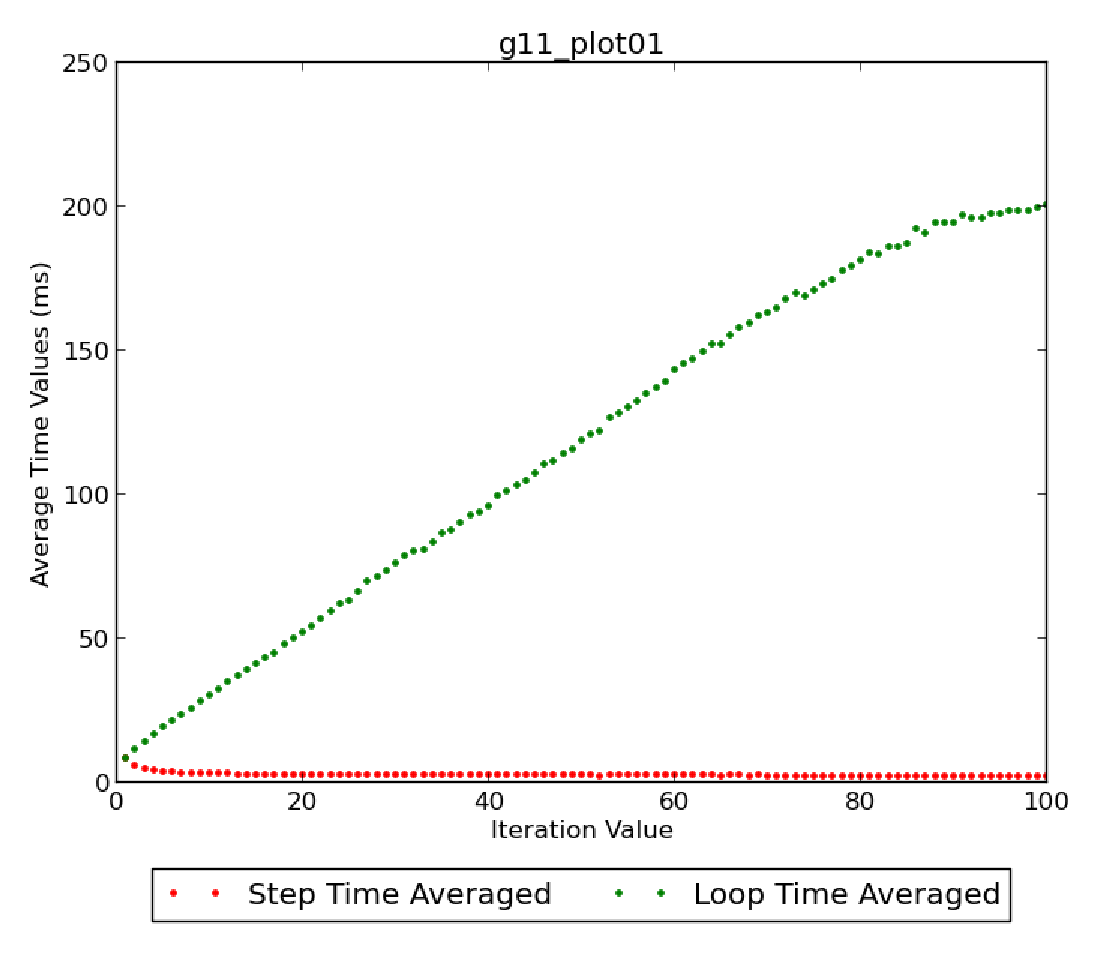
\includegraphics[width=0.5\textwidth,keepaspectratio]{load_1.eps}
In graphs shown above, we have average step time values and total loop time value over all reruns versus iteration value graph. Left side graph is obtained when program is executed with low CPU load and right side graph is obtained when CPU load is high.
\\\\ 
As expected, loop time increases with iteration value since with increasing number of iteration total calculations also increases. Also, the slope of graph decreases when iteration value is around 30.By running the simulation using single step we see that at the 30th step the big sphere which is initially in air collides with the rotating platform and rebounds. At this point the sphere starts going back and therefore the chances of expected collision decreases as relative velocity of sphere w.r.t. platform is away from platform. Therefore the time taken in analysing collision decreases and hence total time taken decreases. So the slope decreases. After that slope again increases slightly and than again decreases because the sphere after reaching a maximum height starts approaching the plank again and increases chance of collision.
\\\\
From the graph we can observe that the average step time value continuously decreases. It might be because the simulation takes more time at initial steps than at later steps so the average is high initially but after the number of steps increases time decreases. This may happen because when more no. of iteration occurs, CPU might prioritise the program, thus helping in the faster execution. Also Box2D looks for the collision when objects have approaching velocity between them. Therefore, after the collision of sphere and plank approaching velocity becomes negative and rest other things remain same, which results in less time taken for collision analysis and hence resulting in decreased step time.
\\\\
If we do the same experiment with increased load on the CPU and memory then the shape of the graph is almost similar but values of average time increases by some factor proportional to load.
\end{subsection}

\begin{subsection}*{Graph 2}
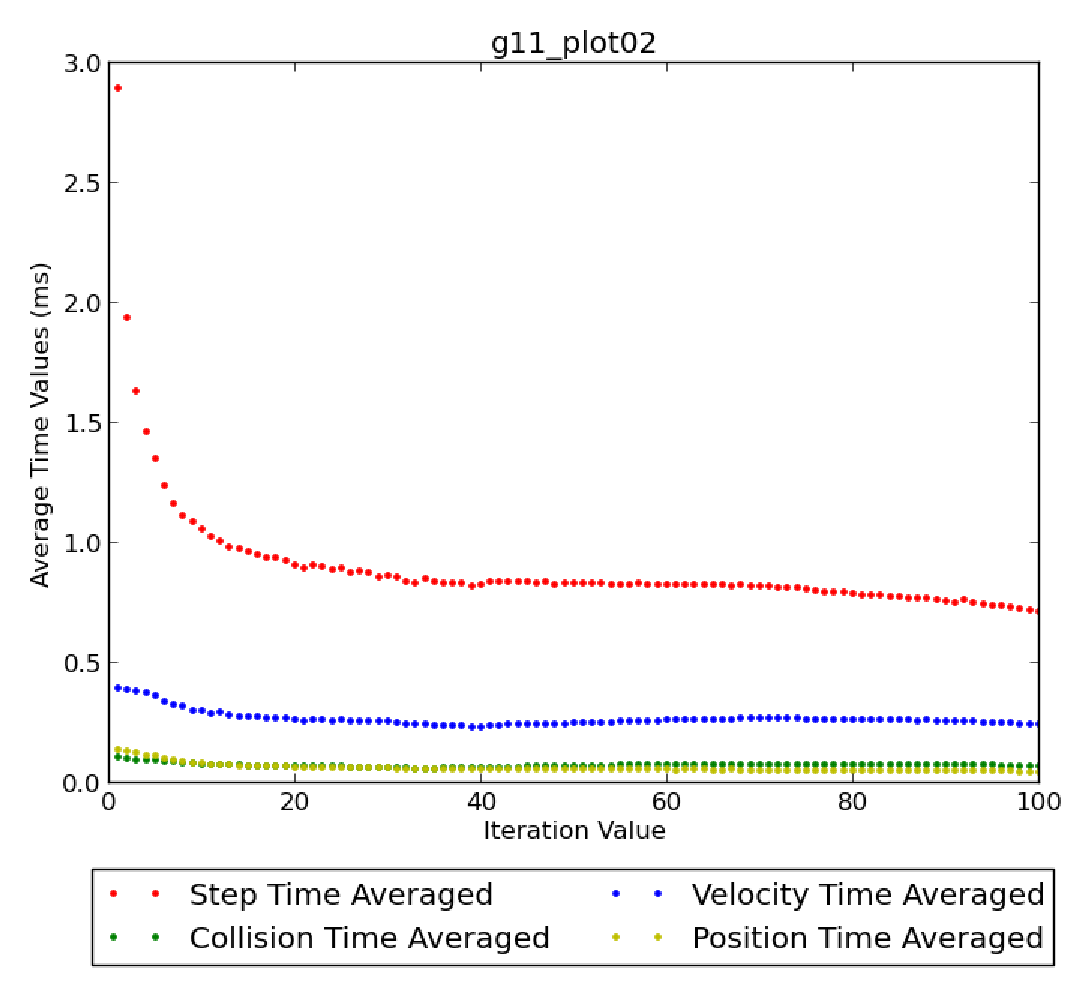
\includegraphics[width=0.5\textwidth,keepaspectratio]{2.eps} 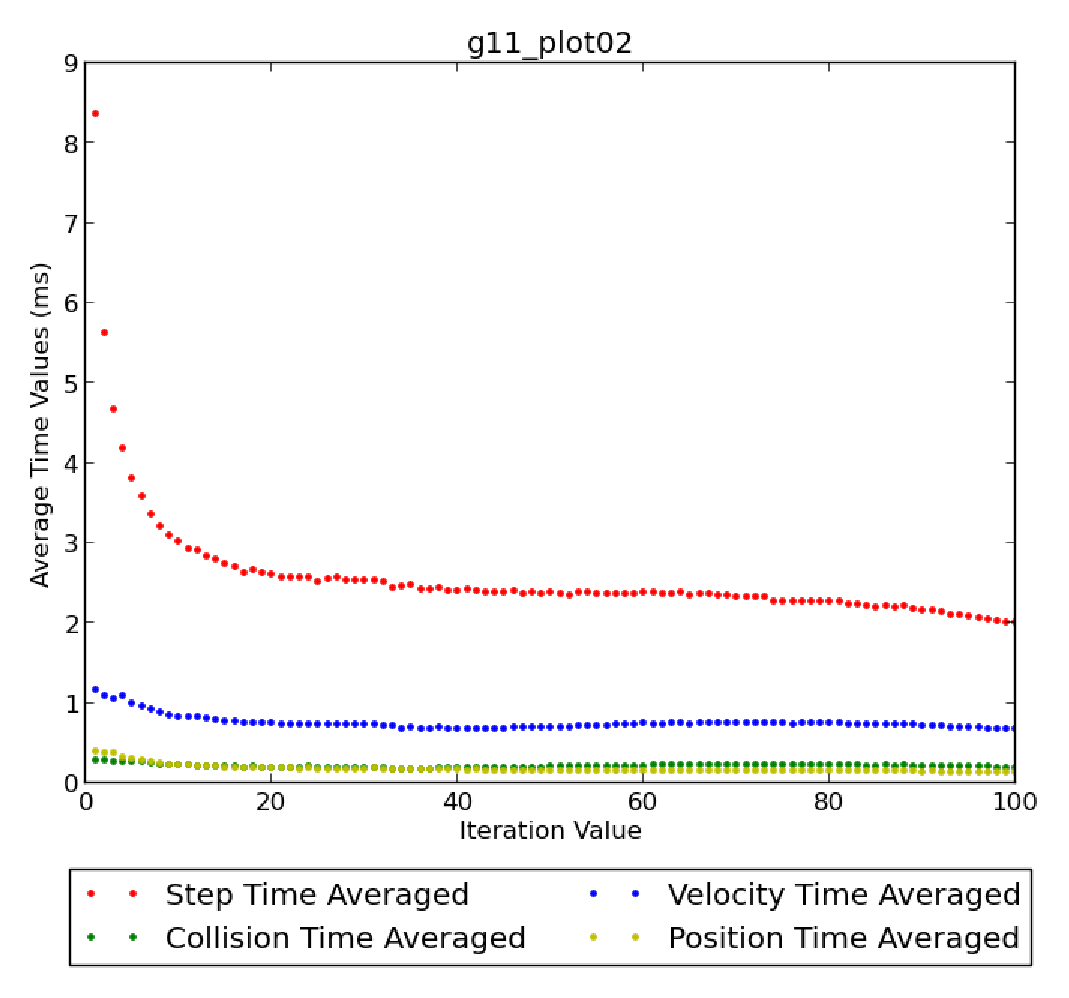
\includegraphics[width=0.5\textwidth,keepaspectratio]{load_2.eps}
In graphs shown above. we have step times, collision detection times, velocity update times and position update times averaged over all reruns versus iteration value of graph.Left side graph is obtained when program is executed with low CPU load and right side graph is obtained when CPU load is high.
\\\\
As observed from Graph 1 average step time decreases continuously with Iteration value.
But the average collision detection times, velocity update times and position update times remains almost constant. Since they only depend on number of steps in simulation and in calculation we have averaged them with the iteration value i.e. number of steps so they remain constant.
\\\\
When load is increased time increases by some factor proportional to load, which is expected as the program will be executed slower. 
\end{subsection}

\begin{subsection}*{Graph 3}
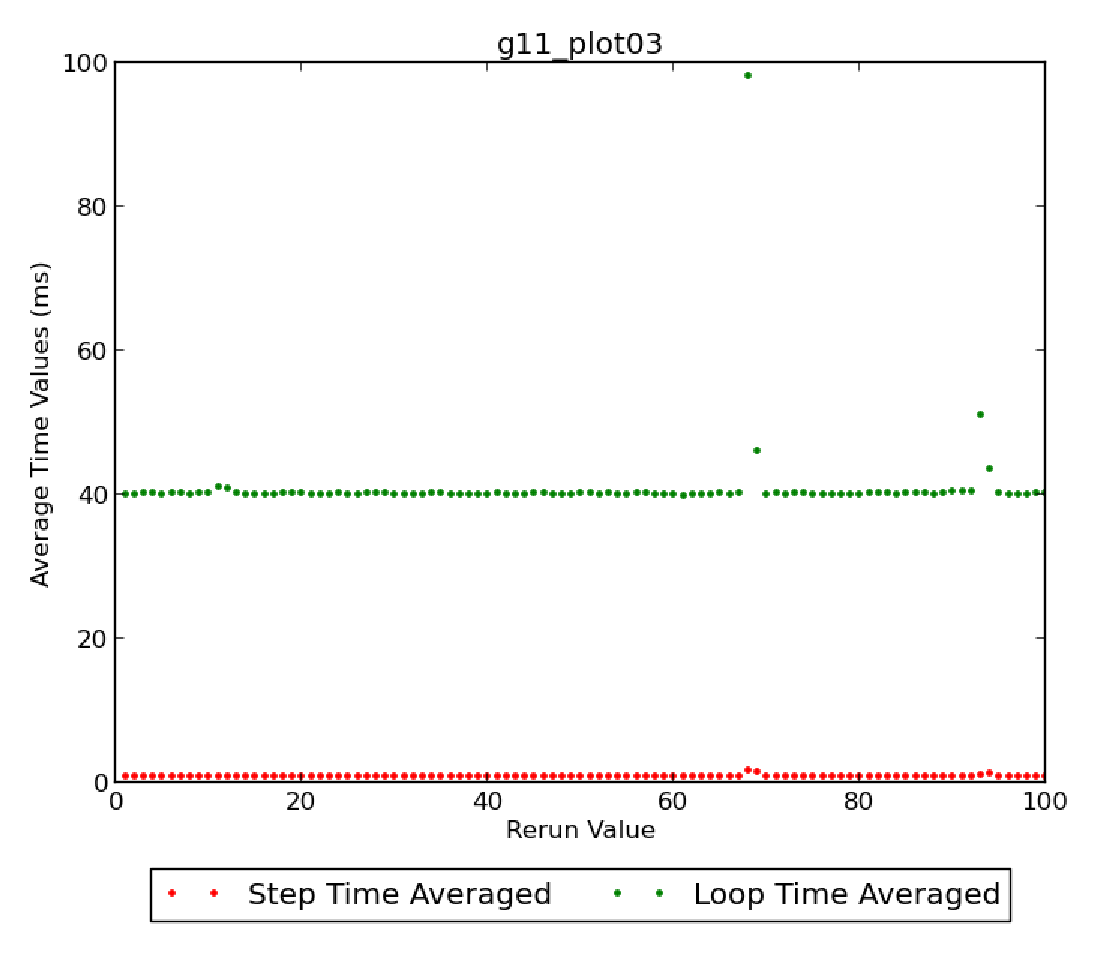
\includegraphics[width=0.5\textwidth,keepaspectratio]{3.eps} 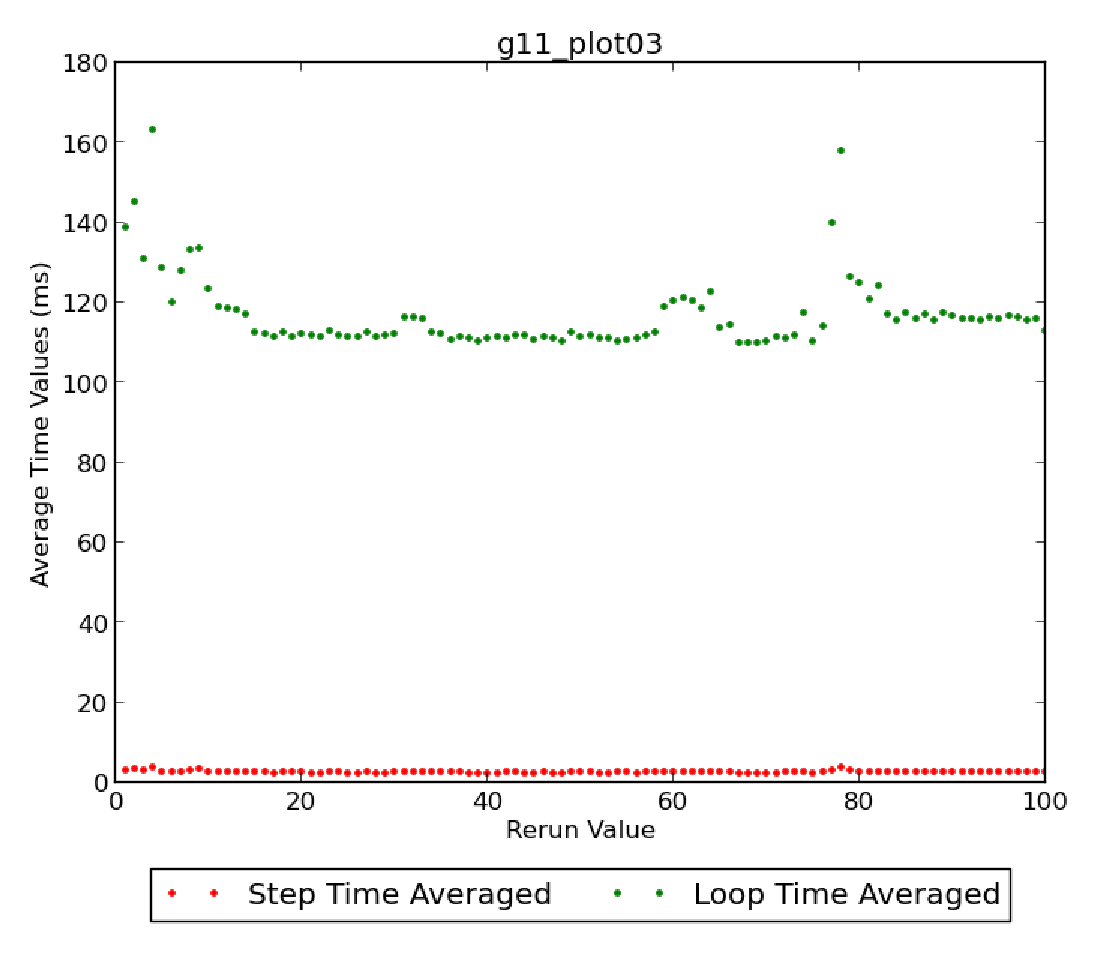
\includegraphics[width=0.5\textwidth,keepaspectratio]{load_3.eps}
In graph 3 we have average step time values and total loop time value over all iterations versus rerun value graph.
We expect both the values to be almost constant with respect to the number of rerun since time of program only depends on iteration value i.e. number of steps and since we averaged it over all iteration value, so values are constant only depending on CPU condition at which rerun is performed.
So when we increase the load it increases the time values according to the load and otherwise it is almost constant. There are some errorneous points due to change in load value in between the running time.
\end{subsection}


\begin{subsection}*{Graph 4}
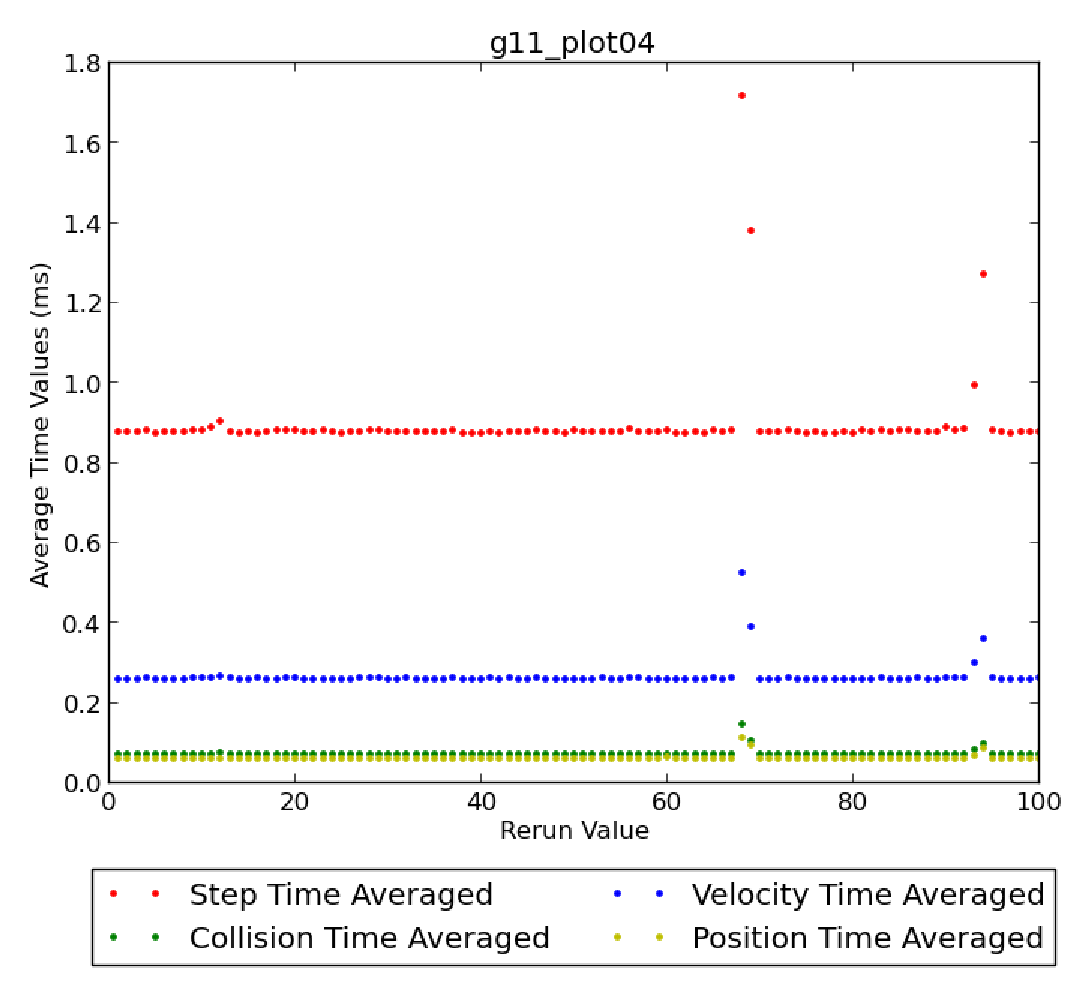
\includegraphics[width=0.5\textwidth,keepaspectratio]{4.eps} 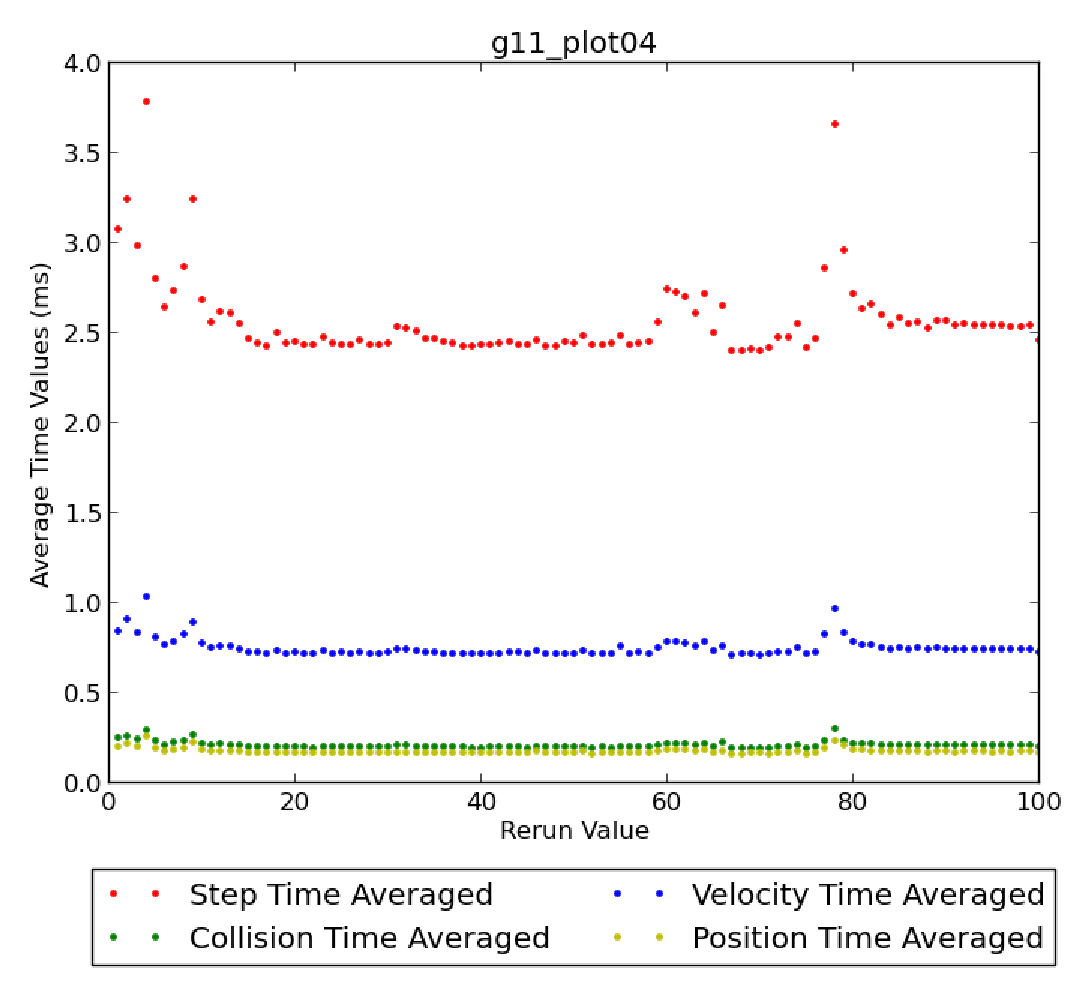
\includegraphics[width=0.5\textwidth,keepaspectratio]{load_4.eps}
In graph 4 we have step times, collision detection times, velocity update times and position update times averaged over all iterations versus rerun value of graph. 
We expect all the values to be constant with respect to the number of rerun since as mentioned above time of program only depends on iteration value i.e. number of steps and we averaged it over all iteration value, so values are constant only depending on CPU condition at which rerun is performed.
So when we increase the load it increases the time values according to the load and otherwise it is almost constant.
\end{subsection}

\begin{subsection}*{Graph 5}
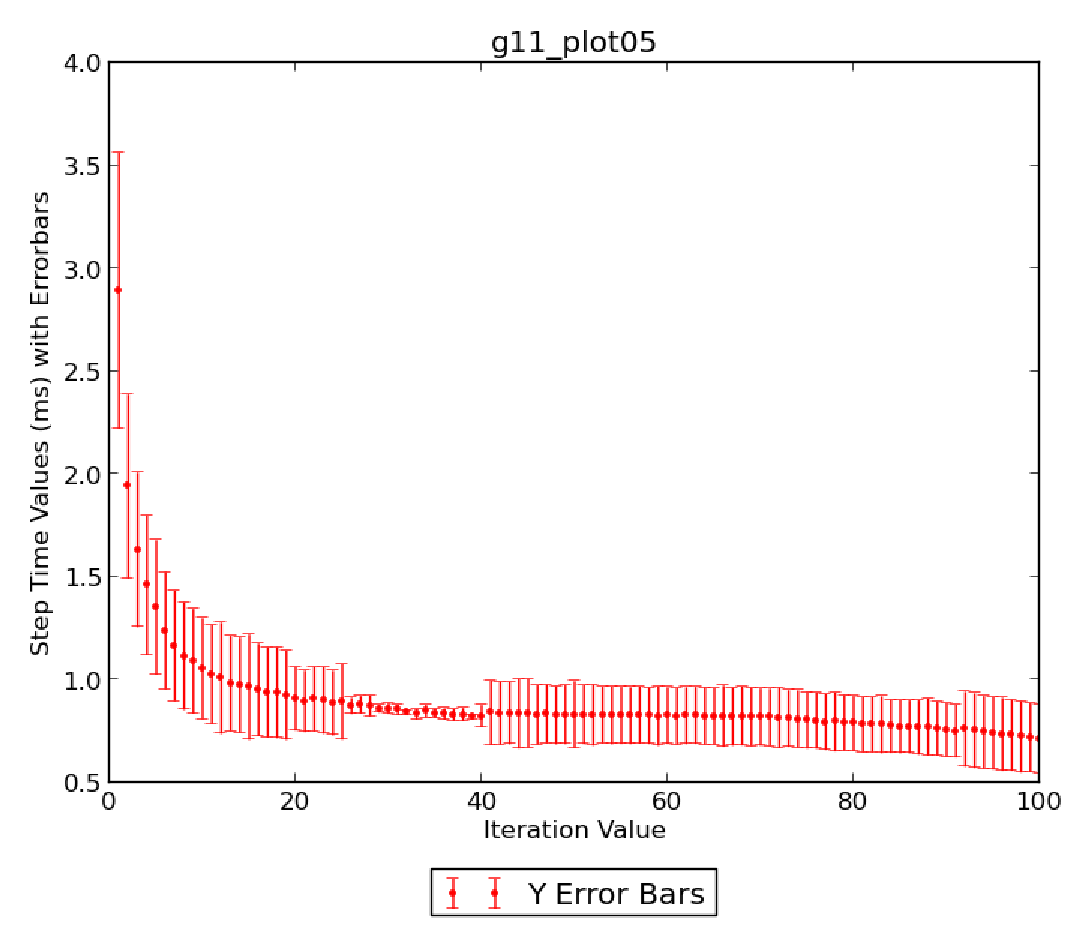
\includegraphics[width=0.5\textwidth,keepaspectratio]{5.eps} 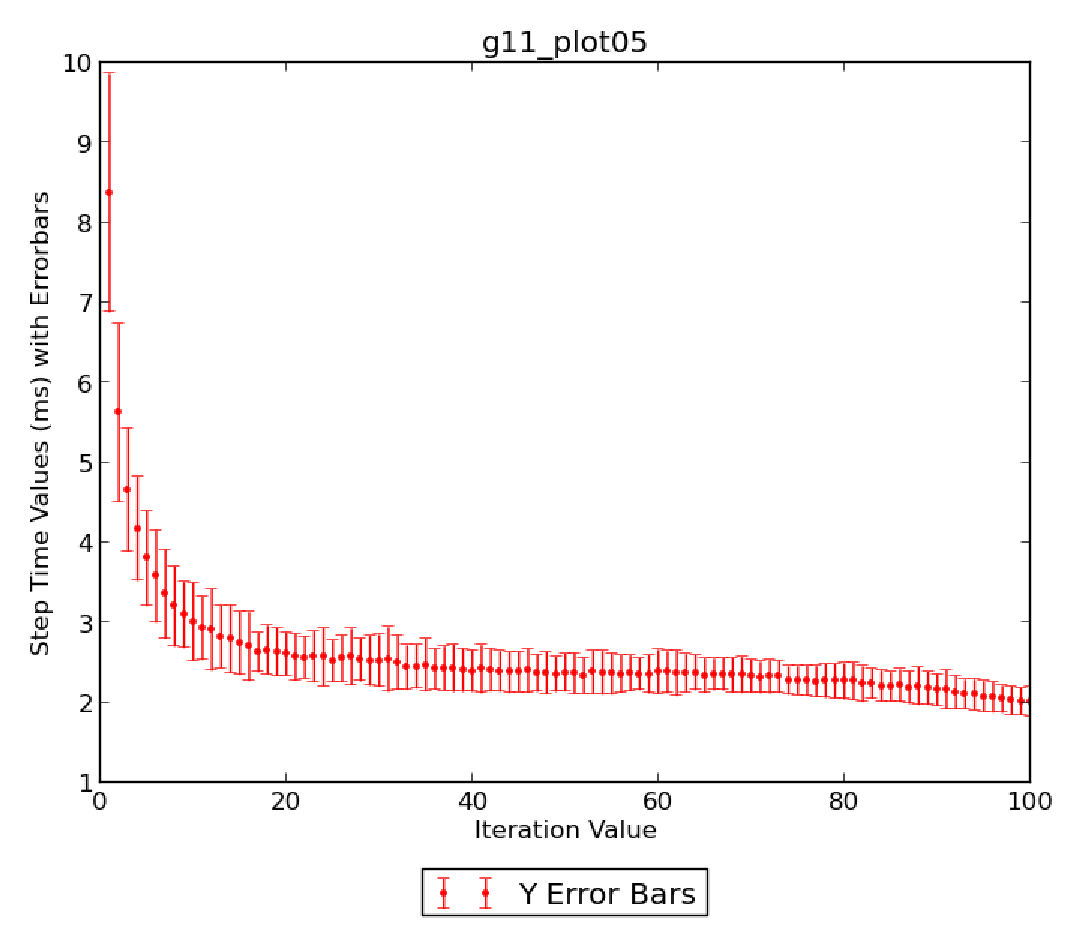
\includegraphics[width=0.5\textwidth,keepaspectratio]{load_5.eps}
In graph 5 we have step time values with error bars according to value at different reruns versus Iteration value.
In most of the cases the error bar is small as there is not much change in values at different reruns of the same iteration value. But at some values error is large it may be due to CPU allocation at some  rerun of that iteration. Because of CPU processing error bars at some points is large. 
With increased load the error bar values also magnifies as the time values also increases. But if we see the relative error it is almost the same with some exceptions due to CPU performance.
\end{subsection}

\begin{subsection}*{Graph 6}
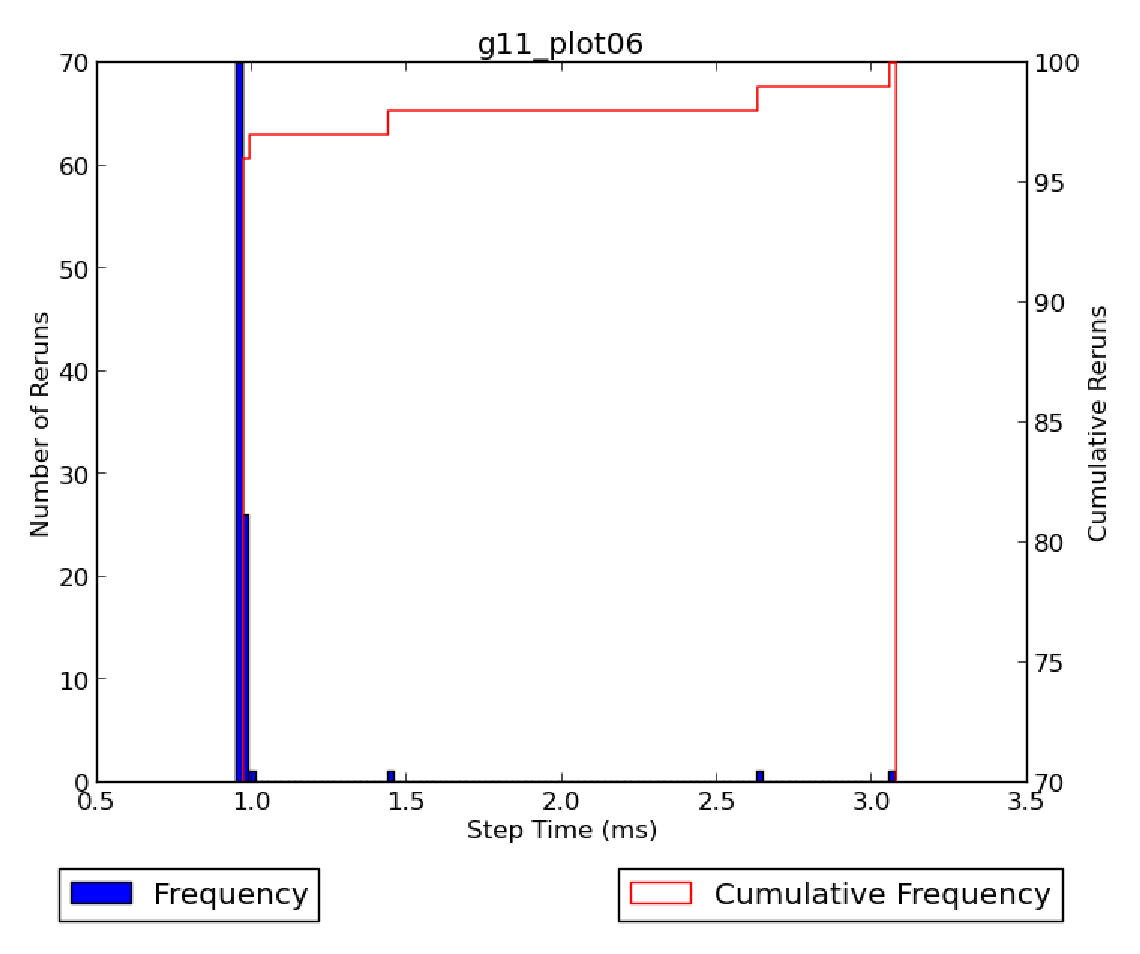
\includegraphics[width=0.5\textwidth,keepaspectratio]{6.eps} 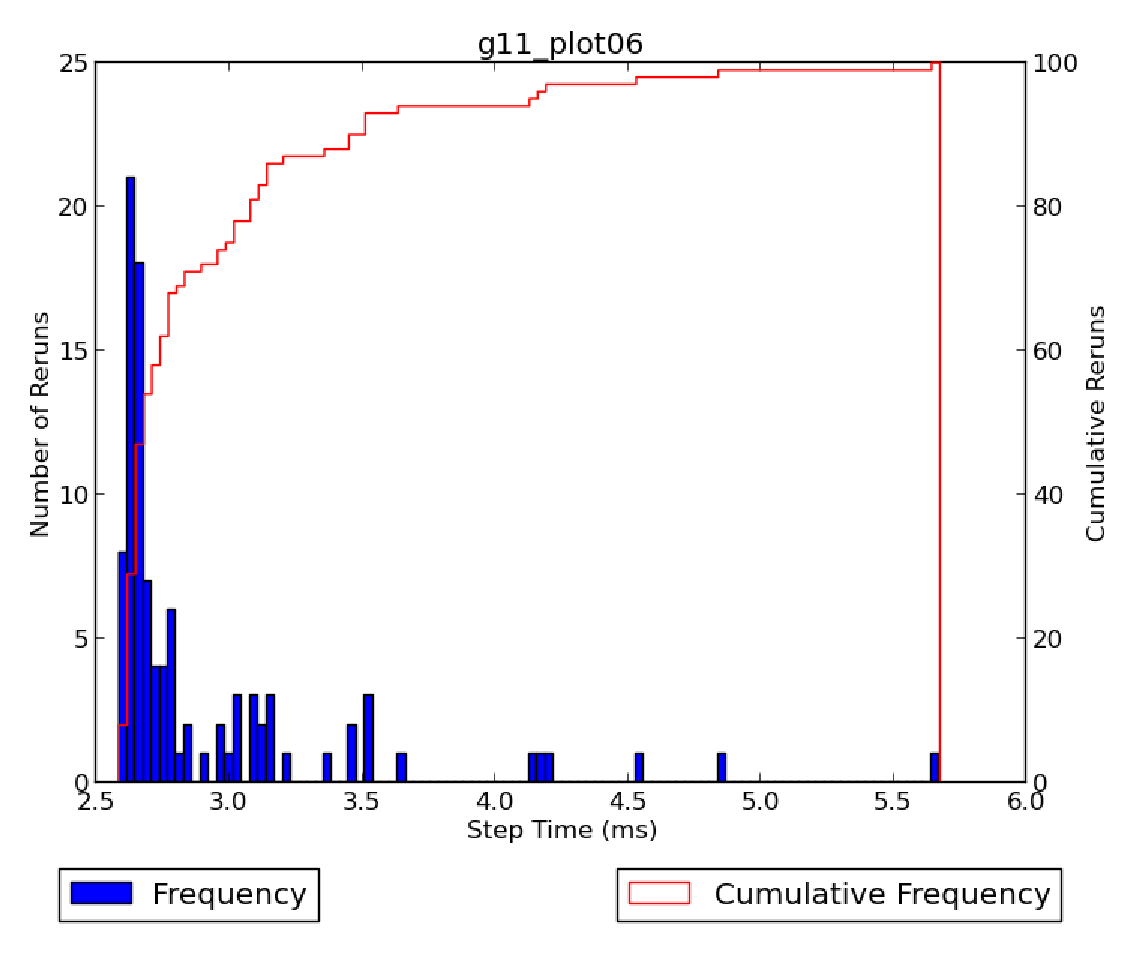
\includegraphics[width=0.5\textwidth,keepaspectratio]{load_6.eps}
In graph 6 we have for a given iteration value frequency and cumulative frequency of reruns with respect to step time
From this graph we can see that most of the reruns occur within some range of steptime and than there are small blocks due to error and CPU processing. Cumulative frequency as expected adds up to 100.
With increased load the distribution of rerun over step time increases i.e. error increases but most of reruns occur in same range of step time.
\end{subsection}

\begin{subsection}*{Comparison between time} 
Time obtained using time command on terminal is more than time obtained using gettimeofday. This is because gettimeofday gives only the time elasped in the running of for loop whereas time obtained from time command includes the time for initialisation of variables along with the execution time of for loop. Latter also includes the time needed to start a program. ~\cite{Time} 
\end{subsection}
\pagebreak

\begin{section}*{Profiling}
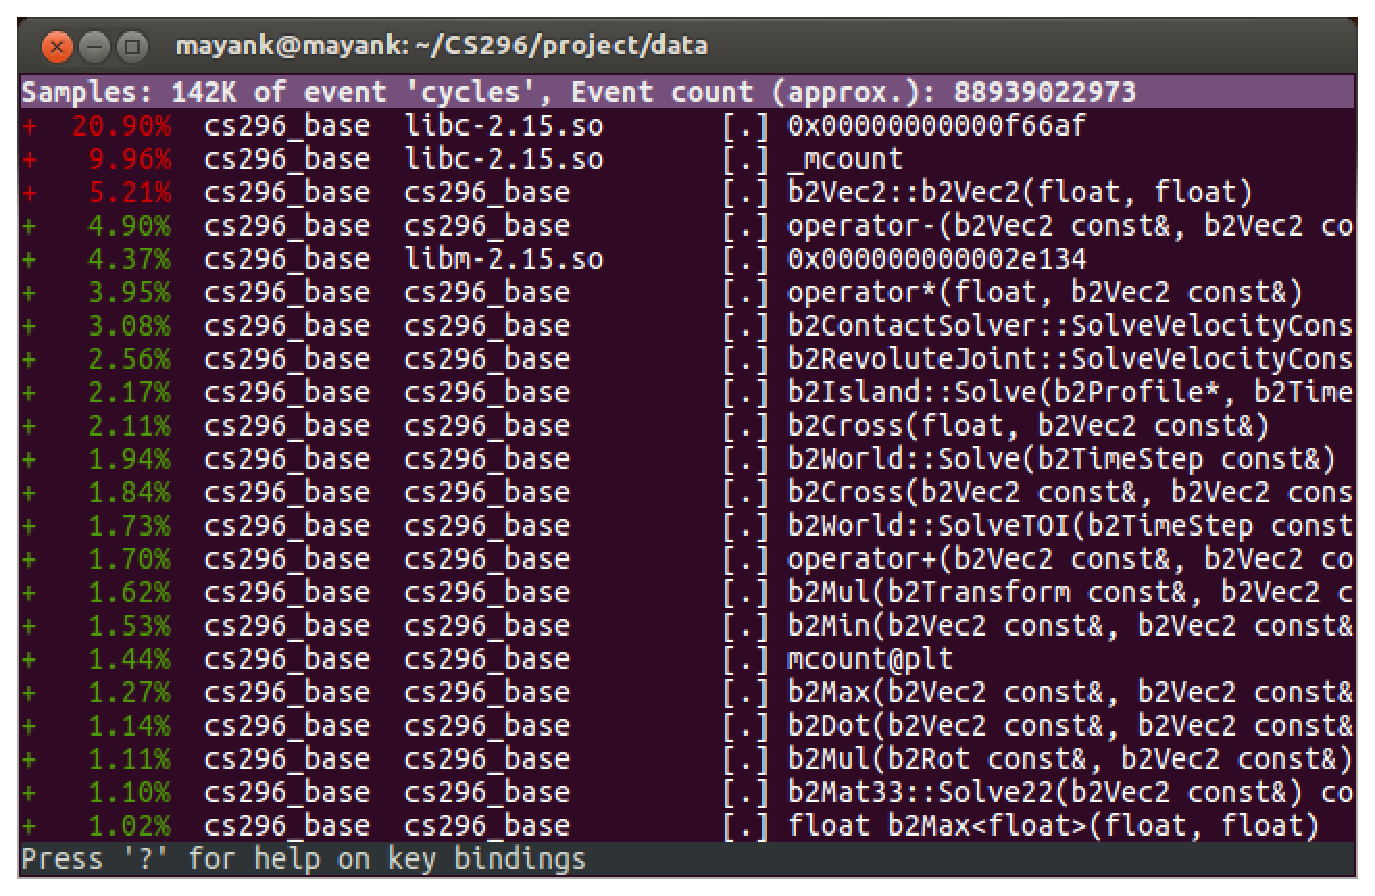
\includegraphics[width=0.5\textwidth,keepaspectratio]{debug.eps} 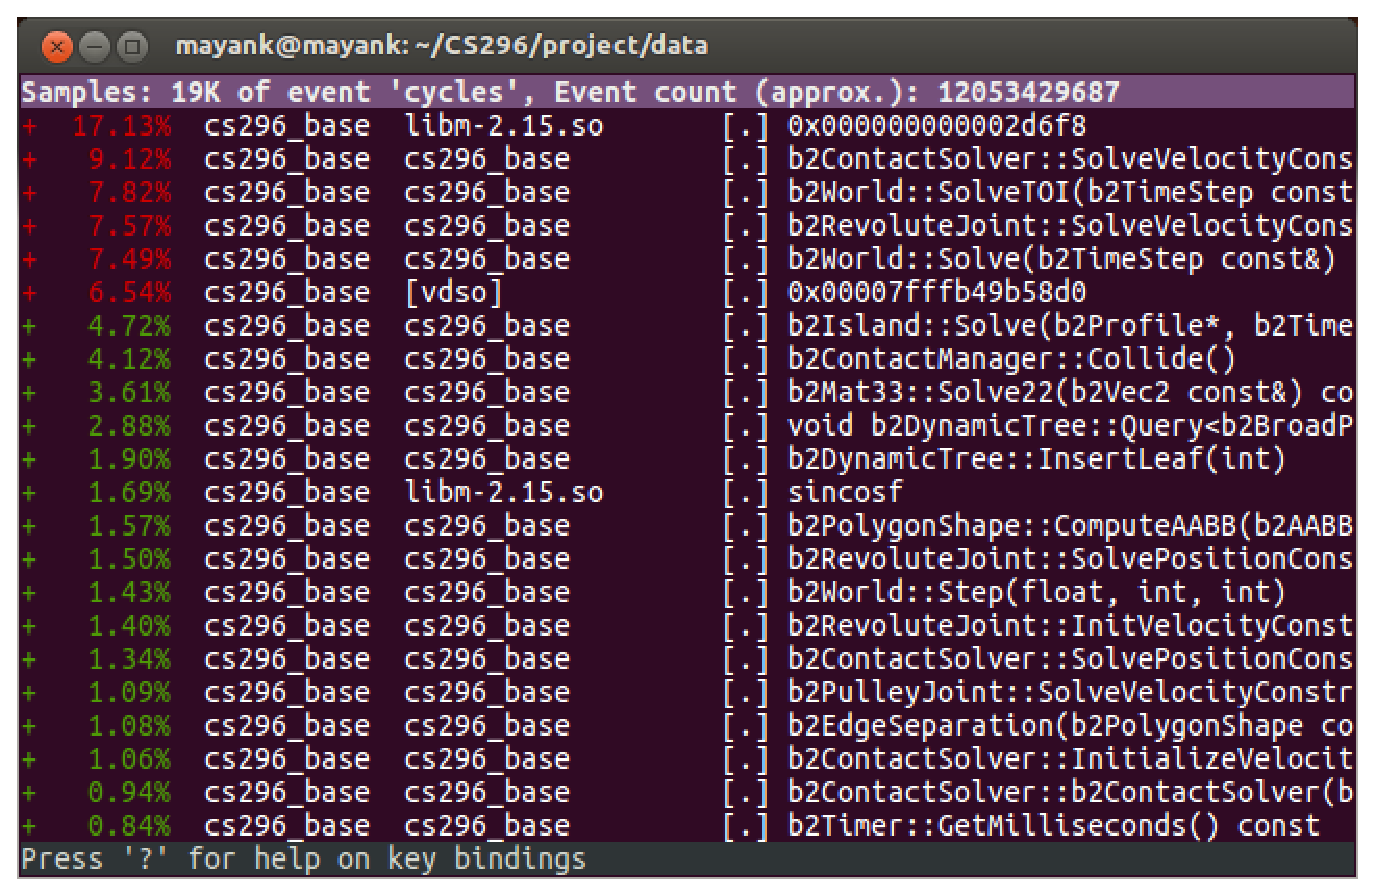
\includegraphics[width=0.5\textwidth,keepaspectratio]{release.eps}
 Profile: \hspace{1in} Debug \hspace{3in} Release
\begin{subsection}*{Choice of no.of iterations value}
For profiling we are running our program for 100,000 iterations, so that when perf is sampling, it doesn't misses the function which are called for very less no. of time or function whose execution time is very less. Also, it will magnify the stats for those function which take very long in their execution or which are called for large no. of times. Also when no. of iterations is less the difference between the time of execution of optimized and non-optimized program isn't visible.~\cite{profiling}
\end{subsection}

\begin{subsection}*{Analysis of optimized and non-optimized program profiles}
 Profiles for both program indicates that SolveVelocityConstrain is the most expensive function. Profile for non-optimized debug mode shows that function like b2Vec2, operator*, operator+ , operator-, b2Cross etc have large no. of calls as they appear in most of the of the calculation and thus they a good toll of total time. But in the optimized profile such function doesn't even appear. In former profile large no. of calls has been made to elementary functions but in the latter profile they have been made inline by -O3 flag of g++ compiler.~\cite{GNU} So calls to such function dosn't appear in latter profile. While using this flag, Compiler heuristically decides which all fuctions to be made inline. Doing this, it avoids many function calls which would have increased the function stack, thus increasing the speed of program. It also unrolls loops in the program which increases the size of executable but increases the speed as it doesn't need to jump from last position to initial position again. Many times a function call is made with same arguments many times, which could be saved into a local variable to avoid repeated function calls.
\\\\
An interesting difference is no. of calls made to function operator* which is of order 8 in debug mode whereas it is negligible in release mode when no. of iterations is of order 6. Even the most expensive function takes about 1.38s in release mode whereas 2.34s in debug mode.  
\end{subsection}

\begin{subsection}*{Suggestion for optimization}
 In b2ContactSolver.cpp, various optimisation could be made. For instance in function SolveVelocityConstraints(), reference to vc$\rightarrow$points is made repeatedly in a for loop, which can be avoided if it is saved in a local variable. Also variables are declared inside the loop which gets redeclared in every iteration of that loop, resulting in the allocation and deallocation of the memory to that variable in each iteration. This could be avoided if variable is declared outside the loop, thus saving the time used in reallocation of memory which is huge.For instance 'vc' is a variable of type b2ContactVelocityConstraint* declared in line 141 inside a for loop, which could have been made better by declaring the same variable outside the loop.  Also unrolling of loop and using local variable could save us a lot of time in many files.
\end{subsection}

\begin{subsection}*{Interpretation From Call Graph}

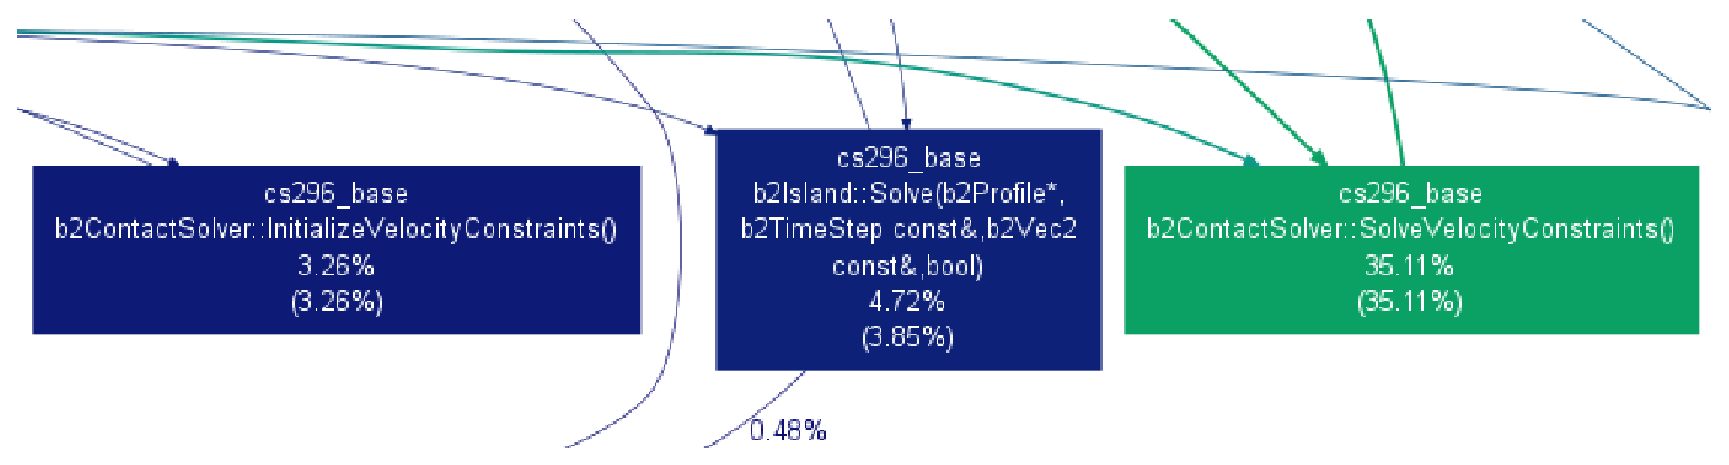
\includegraphics[width=0.9\textwidth,keepaspectratio]{release1.eps} 
\newline \newline
This graph is for release mode. Most expensive function is SolveVelocityConstraints().
\newline \newline
 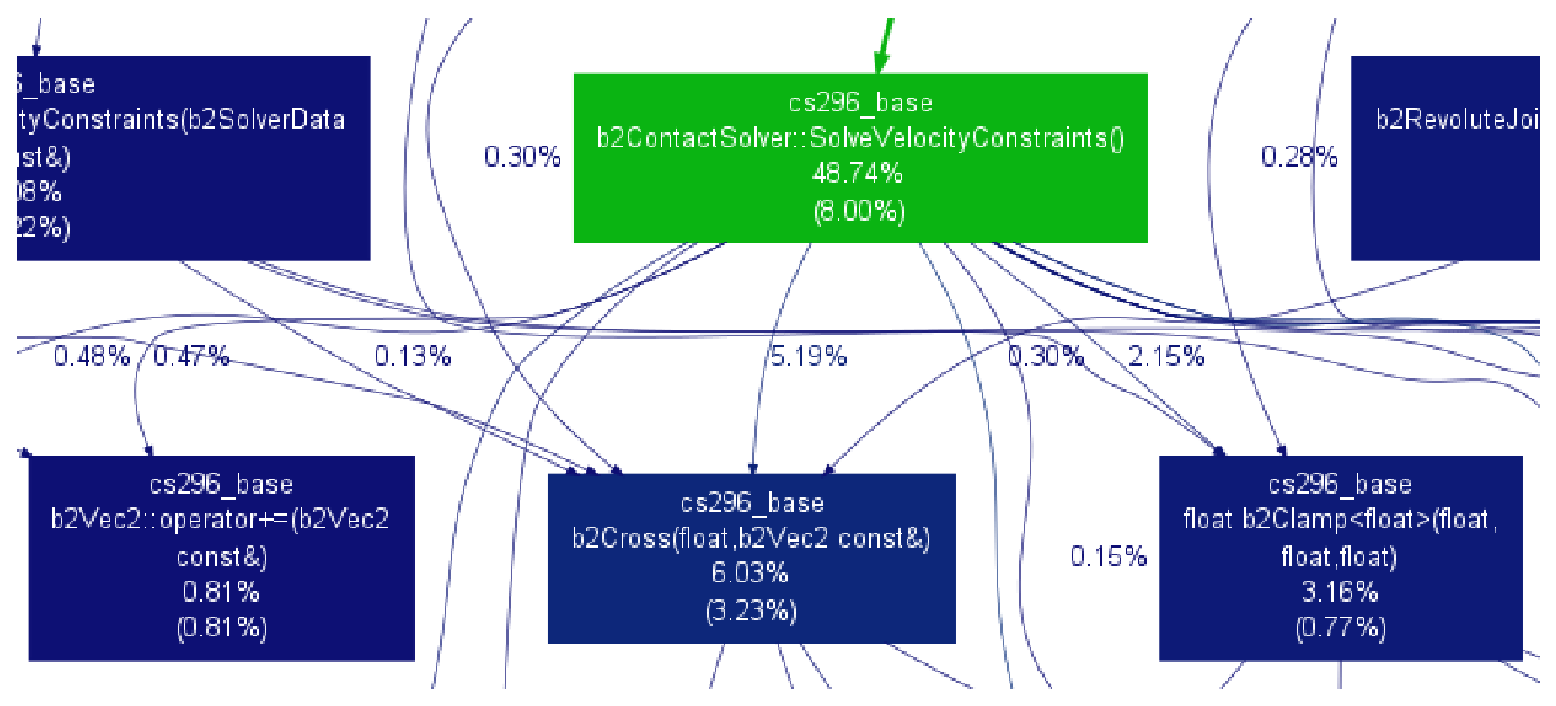
\includegraphics[width=0.9\textwidth,keepaspectratio]{debug1.eps}
 \newline \newline
This graph is for debug mode. Most expensive function is SolveVelocityConstraints(). Also function like b2Cross contributes 6 \%  of the total time whereas such function doesn't even appear in the graph for release mode because of inlining of functions. ~\cite{Perf}
\\\\  
 From callgraph we can see the percentage time taken by each function call and percentage time taken by self. There are arrows emerging from each block which are pointing towards different function blocks and it also indicates the no. of times the pointed function is called from the given function. Each block also has a color code according to its percentage red for high, blue for normal etc. 
\\\\
When we compare the two call graphs one of debug and other of release there is significant change in number of function block as release mode makes many functions inline. Also time of many functions in the release mode decreases when copmpared with debug mode profile which is expected as optimization includes unrolling of loops, using temporary variables, inlining of the functions.
\end{subsection}

 

\end{section}

\bibliographystyle{plain}
\bibliography{g11_prof_report}
\end{document}
